\chapter{Progettazione di una base di dati}

Progettare una base di dati non è un compito semplice. Progettare una base di dati richiede più fasi finalizzate a raccogliere e raccontare la realtà in modo che sia semplicemente accessibile

Le fasi tecniche sono:
\begin{enumerate}
    \item Studio di fattibilità
    \item Raccolta e analisi dei requisiti
    \item progettazione delle funzionalità e dei dati manipolati
    \item Realizzazione
    \item Validazione e collaudio
    \item Funzionamento
\end{enumerate}

A grandi linee le due fasi che si hanno quando si progetta una base dati sono l'analisi e la progettazione vera e propria. Durante la fase di analisi si lavora relativamente alla progettazione concettuale. Durante la fase di progettazione vera e propria si lavorerà invece al modello logico e al modello fisico.

Nell'analisi si vede quindi "\textbf{che cosa si modella}", nella progettazione si vede il "\textbf{come si modella}"

\section{Lo schema ER}

Lo schema Entità Relazione è la visualizzazione più usata per rappresentare una base dati. Questo modello verrà utilizzato per rendere grafico lo schema concettuale e lo schema logico nei passaggi seguenti.


\subsection{I costrutti del ER model}

\paragraph{Entità} Se ha proprietà significative e descrive oggetti con esistenza autonoma.
\paragraph{Attributo} Se è semplice e non ha proprietà.
\paragraph{Relazione} Se correla due o più concetti.
\paragraph{Generalizzazione} Se è caso particolare di un altro.


In questo schema i rettangoli rappresenteranno le entità, le relazioni saranno rappresentate da dei rombi e queste saranno collegate alle entità tramite dei vertici\footnote{Le linee}.

In questo modello sarà importante scegliere \textbf{nomi espressivi} ce siano \textbf{singolari}. Per \textbf{le relazioni} il requisito è lo stesso ma sarà importante \textbf{sostantivarle}.

Queste scelte di nomi saranno utili per comprendere più facilmente cosa si andrà a fare senza forzatamente dare un orientamento alla direzione delle relazioni.

\subsection{Cardinalità delle relazioni e degli attributi}

%Da rivedere
Quando definisco le relazioni e gli attributi dovrò definirne anche la cadinalità, ovvero quante di quelle relazioni possono esserci.


Si definiscono con una coppia di valori tra parentesi, saranno il primo la quantità minima ed il secondo la quantità massima. ad esempio (2,6).

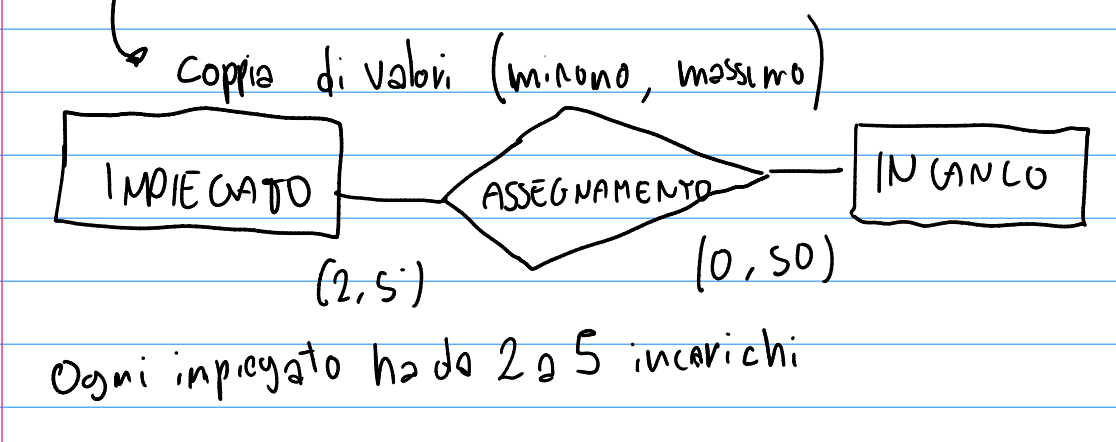
\includegraphics[width = \textwidth]{img/cardinalita_relazioni.png}

solitamente si usano numeri o identificatori come 0,1,n.

Posso definire cardinalità anche relativamente agli attributi.

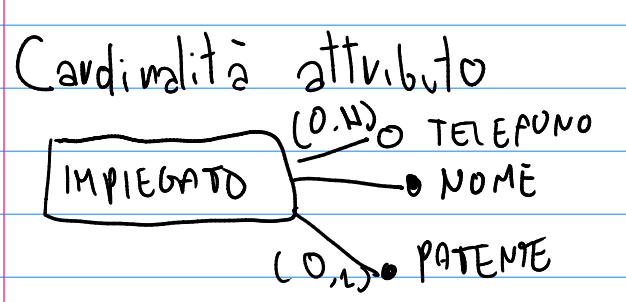
\includegraphics[]{img/cardinalita_attributi.png}

\subsection{Le relazioni}

Esistono vari tipi di relazioni:
\begin{itemize}
    \item binarie
    \item n-arie
    \item ricorsive
\end{itemize}

\paragraph{Relazioni binarie} Una relazione è binaria quando si rapporta a due entità e ne definisce un rapporto.

\paragraph{Relazioni n-arie} Se ho una relazione tra tre\footnote{Ad esempio in questo caso è ternaria} o più entità la relazione sarà n-aria. Un esempio di relazione ternaria è se ad esempio do due volte lo stesso esame avrò tre entità: \textit{persona}, \textit{esame1}, \textit{esame2}

\paragraph{Relazioni ricorsive} Posso avere relazioni ricorsive in molti casi, ad esempio se ho un prodotto che può essere composto da più prodotti ho una relazione ricorsiva con l'entità \textit{prodotto}.

\subsubsection{Gli attributi}

Gli attributi descrivono un' entità. Nel diagramma ER si definiscono con due simboli:

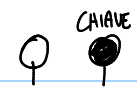
\includegraphics{img/attributi.png}

Il simbolo vuoto indica un'attributo normale, un attributo pieno indica un attributo chiave.

\paragraph{Gli attributi chiave} Un attributo chiave è un attributo che identifica in maniera univoca un oggetto appartenente a quell'entità. Per un cittadino italiano la chiave è il codice fiscale e ogni cittadino è identificato da questa chiave.

\paragraph{Attributi composti} Oltre agli attributi singoli descrivibili semplicemente con il simbolo vuoto posso anche voler descrivere attributi composti, ad esempio un indirizzo è un attributo composto da: Via, numero, cap, città, ecc...


\subsection{Design patterns}
Questi sono alcuni dei design patterns più utilizzati quando si organizza uno schema ER. Questi pattern sono comodi perchè semplificano la creazione e la lettura di un ER graph.

\subsubsection{Reificazione di attributo di entità}
Reificare significa prendere l'astratto per concreto, ovvero considerare concetti, categorie, idee, rapporti astratti alla stregua di oggetti concreti.

In questo caso significa espandere un attributo trasformandolo in entità. Questo è comodo perché ci consente di dare all'attributo altri sotto attributi e in caso di bisogno lo si potrà anche mettere in relazione con altre entità.
\begin{center}
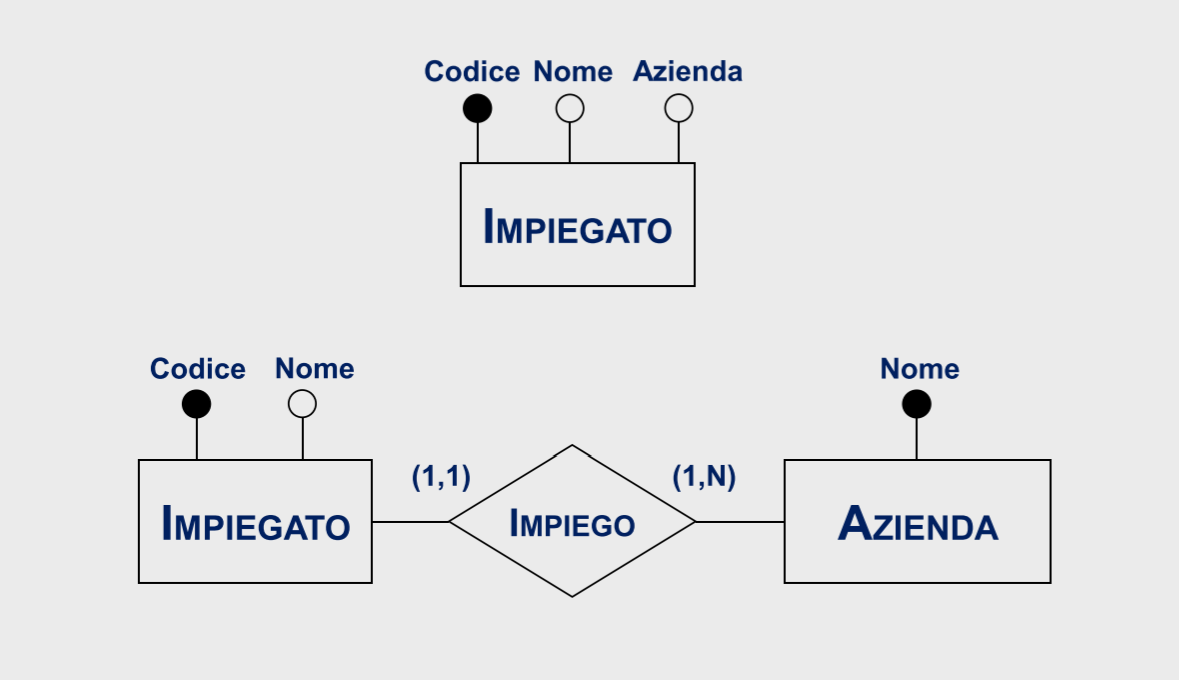
\includegraphics[width=0.5\textwidth]{img/reificazioneDiAttributoDiEntita.png}
\end{center}

\subsubsection{Part-of (Has-a)}
Quando un'entità non può esistere senza una sua sovra-entità, questa entità è "\textit{part-of}" della sovra-entità.

\begin{center}
    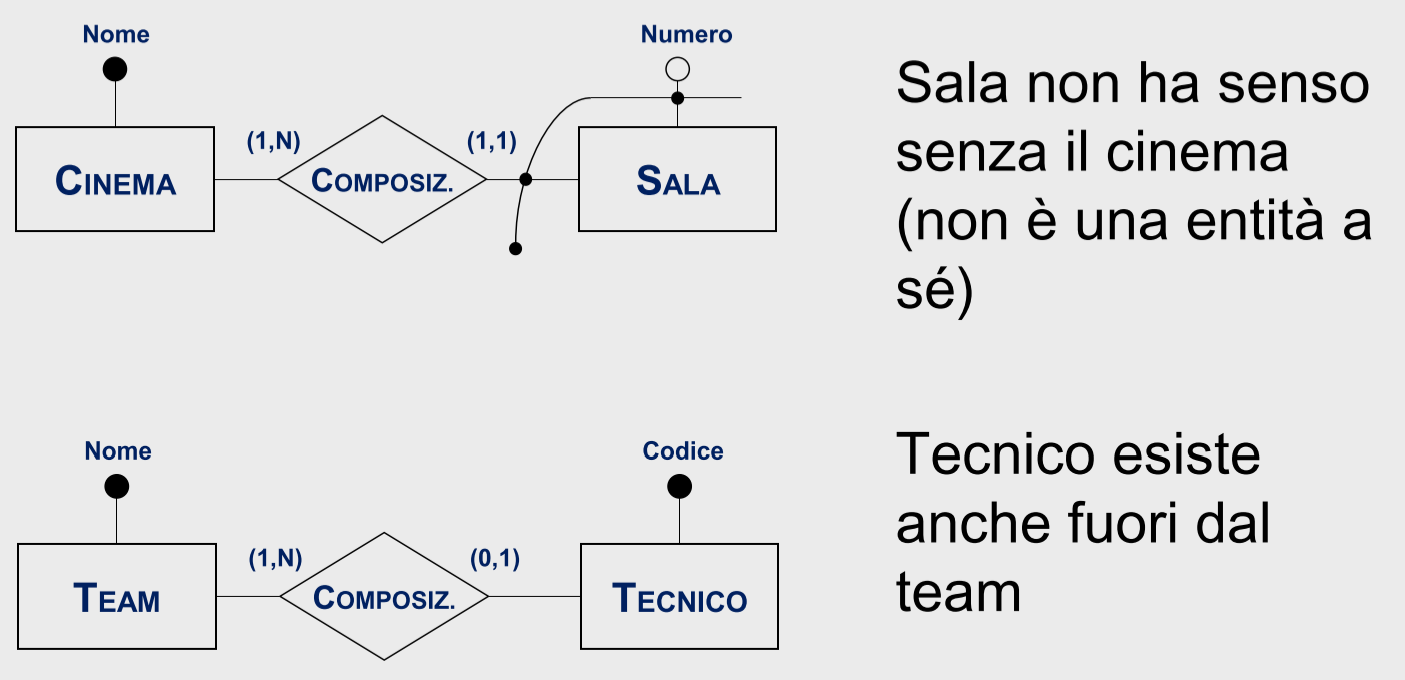
\includegraphics[width=0.7\textwidth]{img/partOf.png}
\end{center}

\subsubsection{Istance-of - Is-a}

Quando un'entità è una specifica versione di un'altra entità è un "\textit{Istance-of}" dell'altra entità.

\begin{center}
    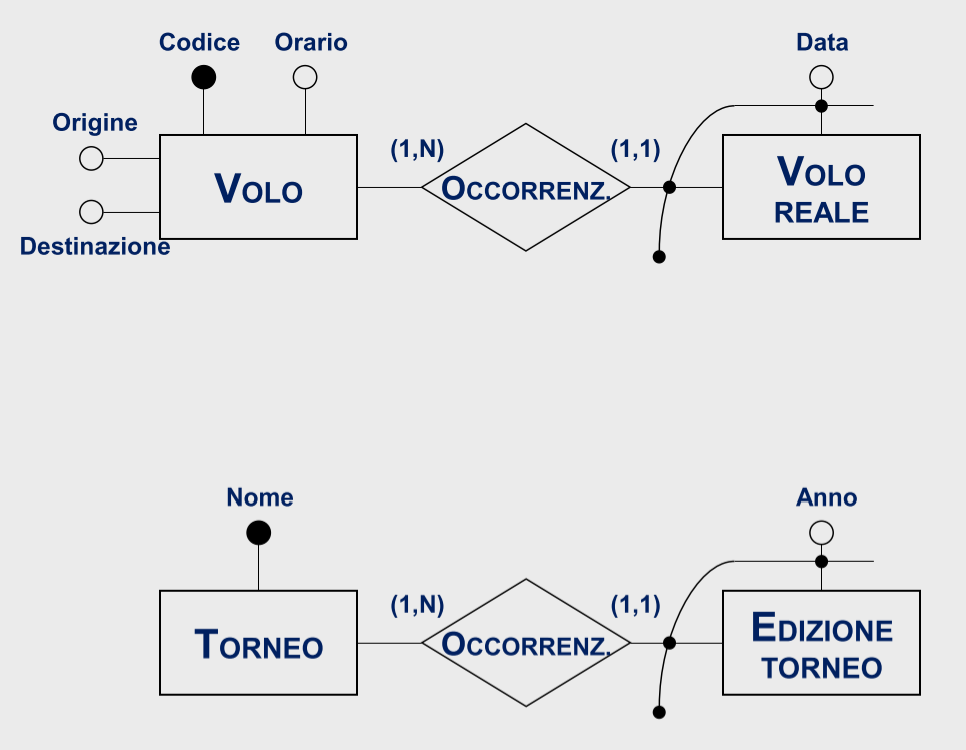
\includegraphics[width=0.7\textwidth]{img/istanceOf.png}
\end{center}

\subsubsection{Reificazione di relazione binaria}

\begin{center}
    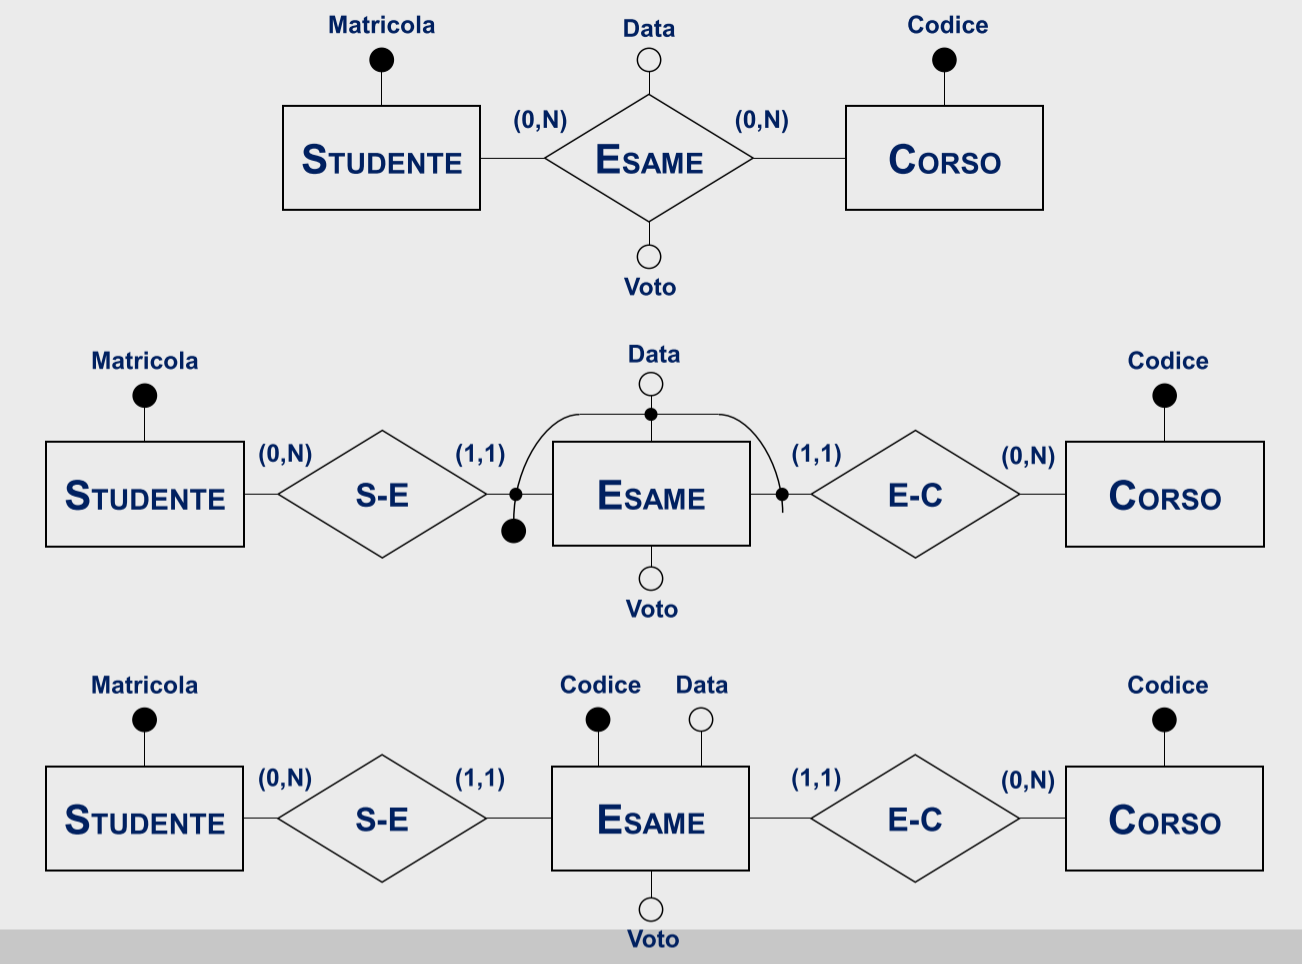
\includegraphics[width=0.7\textwidth]{img/reificazioneDiRelazioneBinaria.png}
\end{center}

\subsubsection{Reificazione di relazione ricorsiva}

\begin{center}
    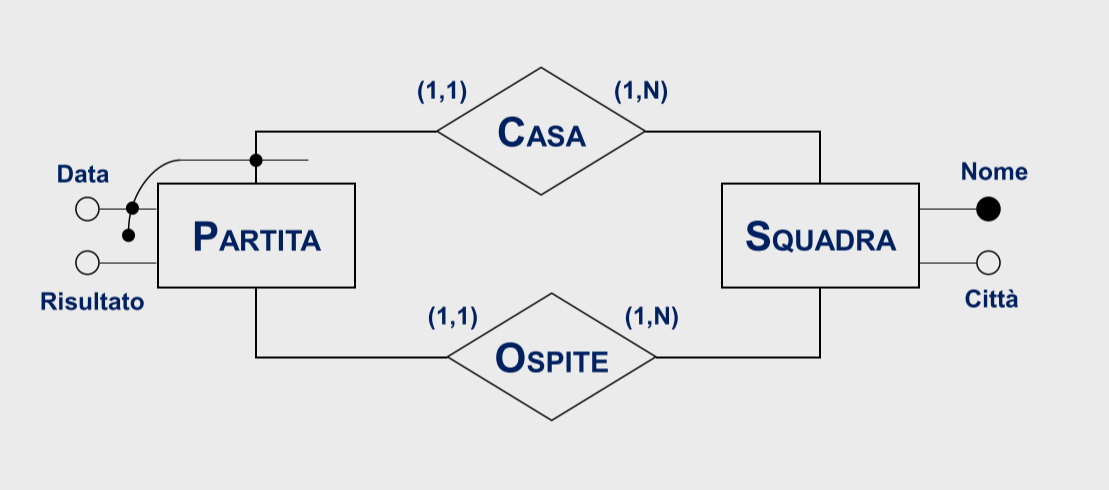
\includegraphics[width=0.7\textwidth]{img/reificazioneDiRelazioneRicorsiva.png}
\end{center}


\subsubsection{Reificazione di attributo di relazione}

\begin{center}
    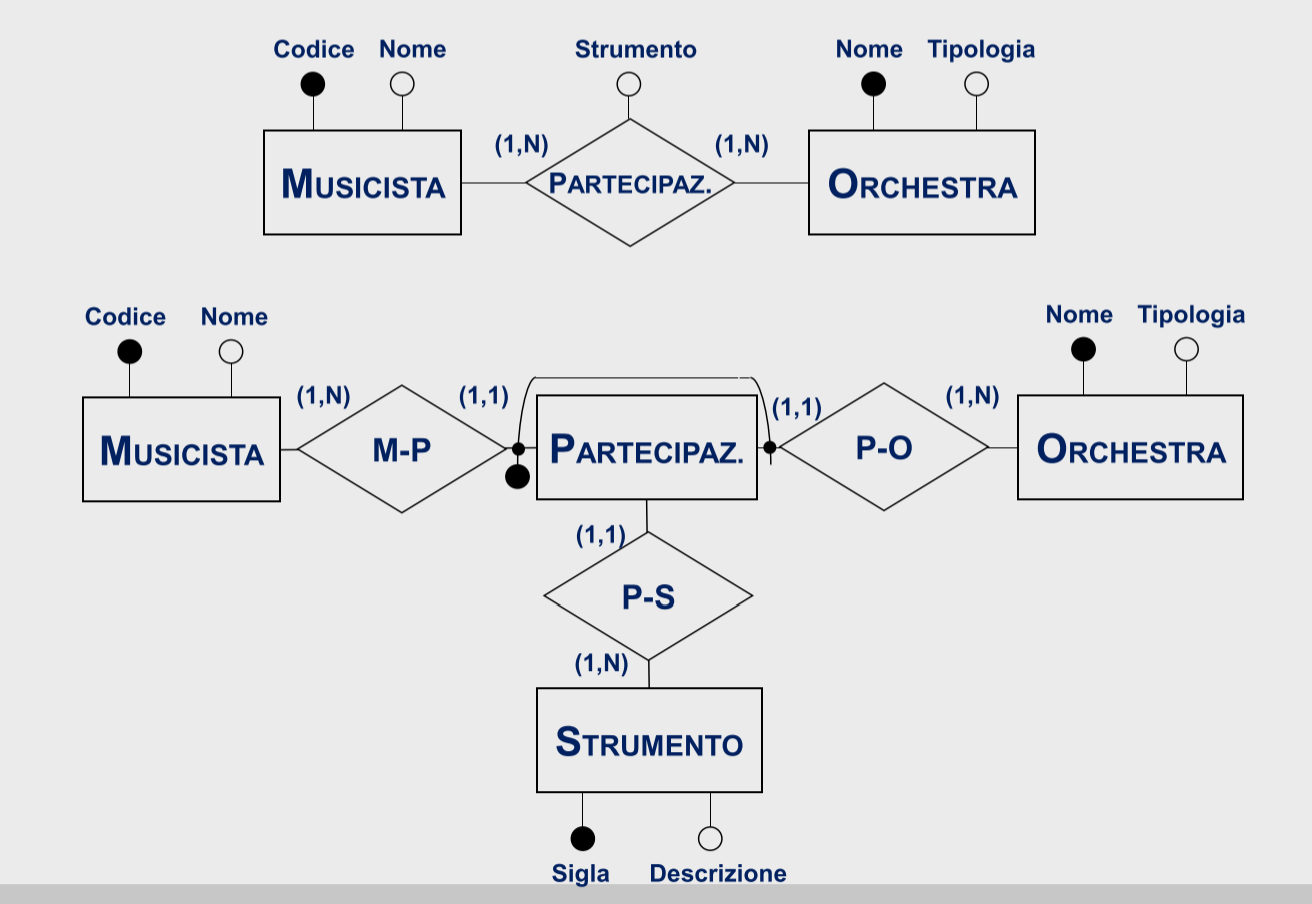
\includegraphics[width=0.7\textwidth]{img/reificazioneDiAttributoDiRelazione.png}
\end{center}

\subsubsection{Caso particolare}


\begin{center}
    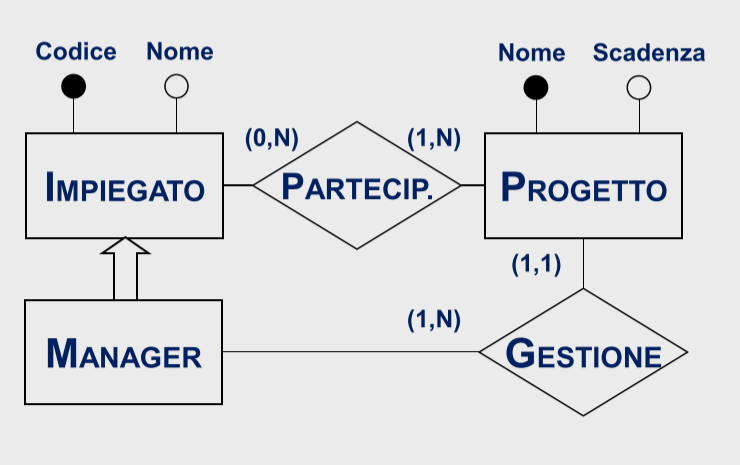
\includegraphics[width=0.7\textwidth]{img/casoParticolare.png}
\end{center}
\subsubsection{Storicizzazione di un concetto}

\begin{center}
    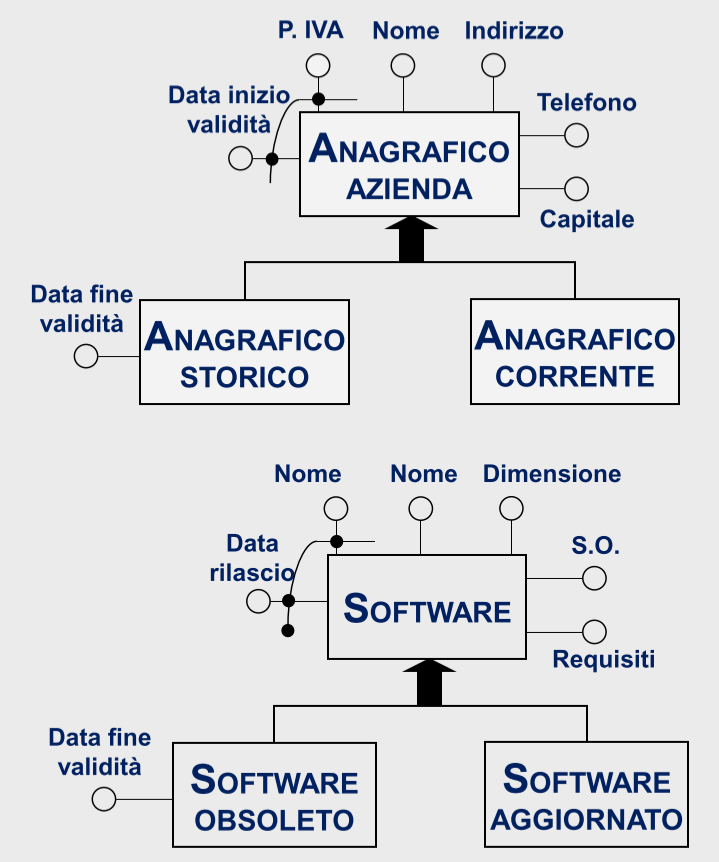
\includegraphics[width=0.7\textwidth]{img/storicizzazioneDiConcetto.png}
    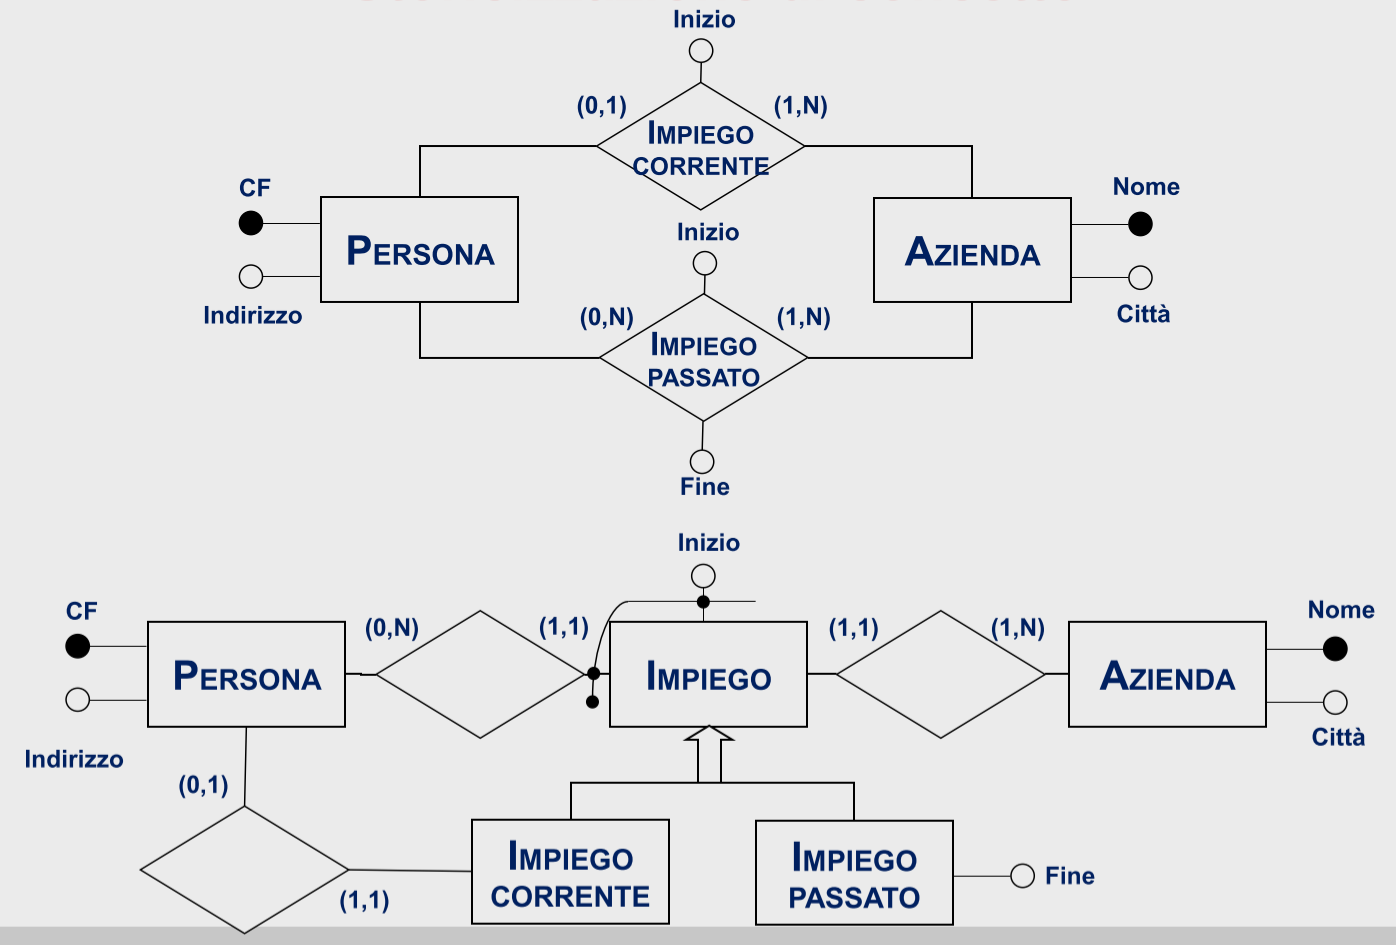
\includegraphics[width=0.7\textwidth]{img/storicizzazioneDiConcetto2.png}
\end{center}

\subsubsection{Evoluzione di un concetto}

\begin{center}
    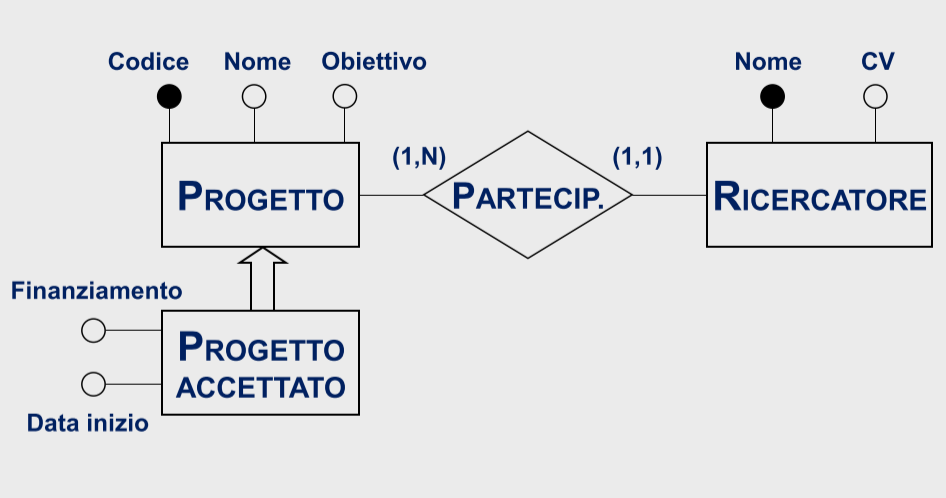
\includegraphics[width=0.7\textwidth]{img/evoluzioneDiConcetto.png}
\end{center}

\subsubsection{Relazione ternaria}

\begin{center}
    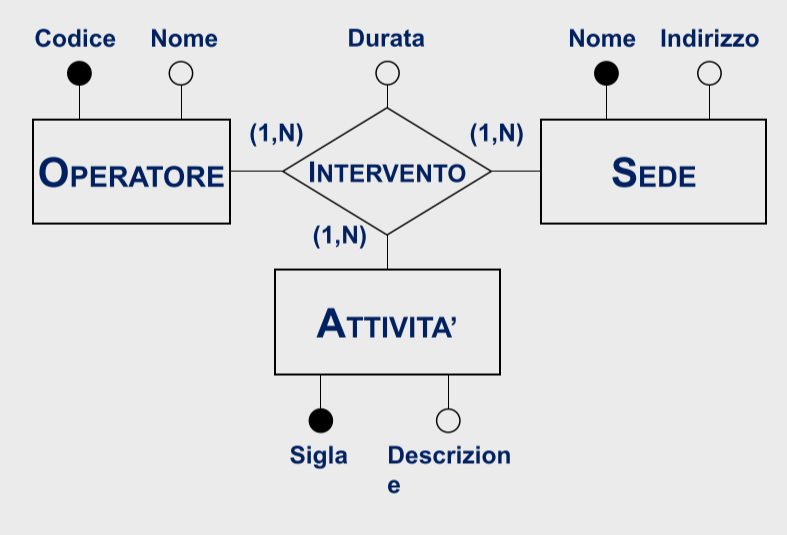
\includegraphics[width=0.7\textwidth]{img/relazioneTernaria.png}
\end{center}

\subsubsection{Reificazione di relazione ternaria}
\begin{center}
    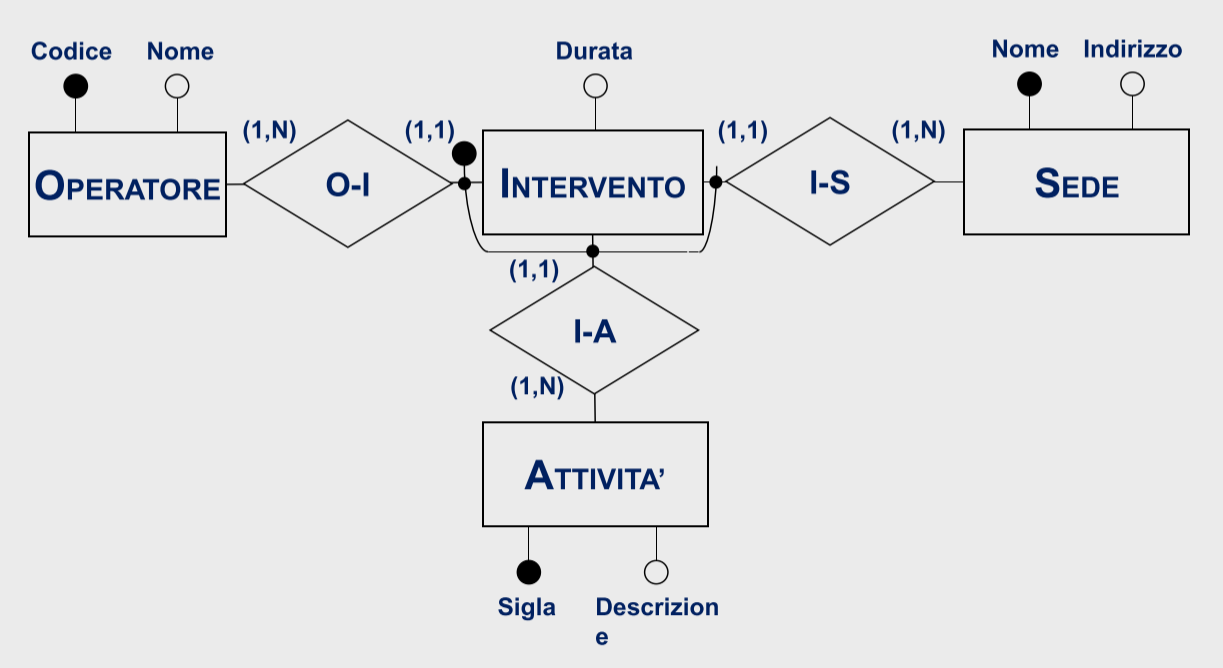
\includegraphics[width=0.7\textwidth]{img/reificazioneDiRelazioneTernaria.png}
    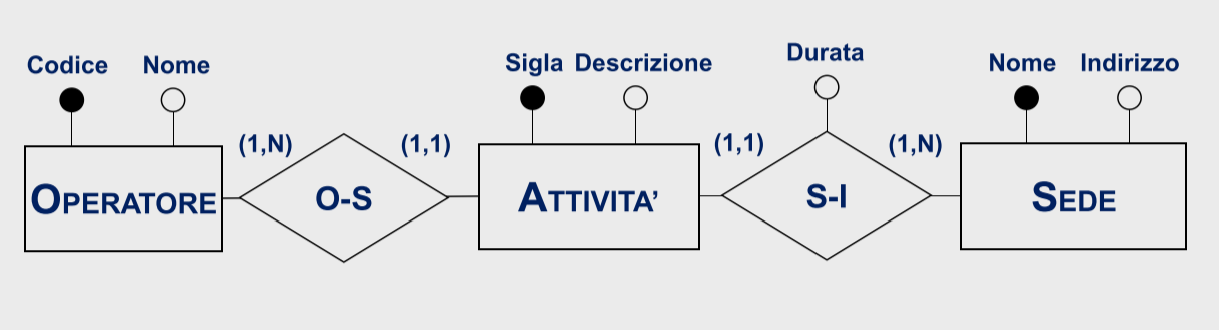
\includegraphics[width=0.7\textwidth]{img/reificazioneDiRelazioneTernaria2.png}
\end{center}

\section{Analisi}

Durante questa fase, lo scopo è quello di comprendere al meglio e nella maniera più aderente possibile cosa si dovrà modellare poi nelle fasi successive. I passaggi sono inquadrati nel seguente modo:

\begin{enumerate}
    \item Acquisizione dei requisiti
    \item Analisi dei requisiti
    \item Costruzione dello schema concettuale
    \item Costruzione del glossario
\end{enumerate}

In questa fase devo quindi acquisire i requisiti per la realizzazione, analizzare i dati raccolti e dovrò da queste informazioni ottenute generare uno schema relazionale ed un glossario dei termini.

\subsection{Acquisizione dei requisiti}

Questo è il momento in cui dovrò ascoltare utenti e committenti attraverso interviste o attraverso la lettura di documentazione precedentemente redatta.

Esempi di documenti da analizzare sono realizzazioni preesistenti e procedure aziendali.

Inoltre è poi importante controllare fonti, documentazioni, leggi e regolamenti.

Il reperimento dei requisiti è un'attività critica, complessa e non standardizzabile. Esistono però delle regole generali che conviene seguire.

\begin{itemize}
    \item Scegliere il corretto livello di astrazione
    \item Standardizzare la struttura delle frasi
    \item Suddividere le frasi articolare
    \item Separare le frasi sui dati da quelle sulle funzioni
    \item Costruire un glossario dei termini
    \item Individuare omonimi e sinonimi
    \item Rendere esplicito il rifermento tra termini
    \item Riorganizzare le frasi per concetti
\end{itemize}



\subsection{Progettazione concettuale}

È importante iniziare da una progettazione concettuale e quindi da uno schema concettuale poiché è importante avere a mente e chiarire in maniera solida e visiva quelli che sono i concetti che dovremo memorizzare nella base dati.

Se iniziassimo subito a mettere mano alle componenti specifiche delle basi di dati sarebbe difficile capire da dove iniziare e si rischierebbe di perdersi, infatti il modello logico ha molto focus sui dati e la rappresentazione delle relazioni e delle classi.

Il modello concettuale serve a ragionare sulla realtà di interesse indipendentemente dagli aspetti realizzativi. Questo ci permette di visualizzare quella che è la realtà in maniera schematica e chiara.

Il modello concettuale permette di rappresentare le classi di oggetti di interesse e le loro correlazioni.

Lo schema che utilizzeremo per rappresentare il modello sarà uno schema \textbf{ER}\footnote{Entità Relazione}.
